\documentclass[xcolor=table,dvipsnames,table]{beamer}
\mode<presentation>
\usetheme{boxes}
\setbeamertemplate{navigation symbols}{}
% http://www.latex-community.org/forum/viewtopic.php?f=4&t=6694
\setbeamertemplate{navigation symbols}{\raisebox{5pt}{\makebox[\paperwidth]{\hfill\makebox[10pt]{\scriptsize\insertframenumber\vspace{1ex}}}}}
%\setbeamertemplate{footline}[frame number]
\setbeamertemplate{blocks}[shadow=false]
%\setbeamercolor*{block title}{fg=structure,bg=RoyalBlue!10}
\setbeamercolor*{block title example}{fg=structure,bg=RoyalBlue!10}
%\setbeamercolor*{block title example}{fg=BrickRed,bg=Goldenrod!10}
\setbeamercolor*{block title alerted}{fg=white,bg=black}
\addtobeamertemplate{block begin}{\pgfsetfillopacity{0.8}}{\pgfsetfillopacity{1}}
%\rowcolors{0}{RoyalBlue!20}{RoyalBlue!5}
\setbeamertemplate{caption}{\raggedright\insertcaption\par}

%\DeclareGraphicsRule{*}{mps}{*}{}

\usepackage{latexsym}
\usepackage{hyperref}
\usepackage{tikz}
\usetikzlibrary{calc,shapes,arrows,shadows,shapes.callouts,shapes.arrows,chains,positioning,trees}
\usepackage{solution}
\usepackage{calc}
\usepackage{pifont}
\usepackage{algorithmic}
\usepackage{pdfcomment}
\usepackage{color}

\newcommand{\cmark}{\ding{51}}
\newcommand{\xmark}{\ding{55}}

\newcommand{\highlight}[1]{{\color{blue}{#1}}}
\newcommand{\mycite}[1]{{\color{darkgray}{\footnotesize [#1]}}}

\DeclareMathOperator*{\argmin}{arg\,min}
\DeclareMathOperator*{\argmax}{arg\,max}
\DeclareMathOperator{\sign}{sign}
\DeclareMathOperator{\cnt}{Count}

\newcounter{mycallout}

\newcommand{\callouts}[3]{%
  \stepcounter{mycallout}
  \tikz[remember picture,baseline]{\node[anchor=base,inner sep=0,outer sep=0]%
    (\themycallout) {\colorbox{#1!20}{#3}};\pause\node[overlay,rectangle callout,%
    callout relative pointer={(0cm,0.5cm)},fill=#1!20] at ($(\themycallout.south)+(-0cm,-0.7cm)$){#2};}%
    }%

\raggedright

\newcount\lecturecount
\lecturecount=0
\AtBeginLecture{%
    \advance\lecturecount by 1
    \date{}
    \begin{frame}
    \begin{center}
    \titlepage
    \ifnum\lecturecount=1
    Part \the\lecturecount: \insertlecture
    \else
    Part \the\lecturecount: \insertlecture
    \fi
    \end{center}
    \end{frame}
}

\addtobeamertemplate{block begin}{\setlength\abovedisplayskip{0pt}}

%\newcommand{\example}[1]{{\color{BrickRed!50}{#1}}}
\newcommand{\maths}[1]{{\color{RoyalBlue!50}{#1}}}
\newcommand{\reference}[1]{{\color{RoyalBlue!30}\tiny [from #1]}}
\newcommand{\koehnref}{\reference{\href{http://www.statmt.org/book}{P.Koehn SMT book slides}}}


\begin{document}

\title{\color{MidnightBlue}Natural Language Processing}

\author{Anoop Sarkar \\ {\color{RoyalBlue!70}{\href{http://anoopsarkar.github.io/nlp-class}{anoopsarkar.github.io/nlp-class}}}}
\institute{\color{BrickRed}Simon Fraser University}
%\date{}
     
{
\addtocounter{framenumber}{-1}
\begin{frame}
\begin{center}
\vspace{8mm}

\includegraphics[scale=0.35]{figures/natlang-cky-logo}
\end{center}
\titlepage
\end{frame}
}



\lecture{Feedforward neural networks}

\section{Log-linear models versus Neural networks}
\frame{\tableofcontents[currentsection]}

\begin{frame}{Log linear model}
\begin{itemize}[<+->]
\item Let there be $m$ features, $f_k(\textbf{x}, y)$ for $k = 1, \ldots, m$
\item Define a parameter vector $\textbf{v} \in \mathbb{R}^m$
\item A log-linear model for classification into labels $y \in {\cal Y}$: 
\[ \Pr(y \mid \textbf{x}; \textbf{v}) = \frac{exp\left(\textbf{v} \cdot \textbf{f}(\textbf{x}, y))\right)}{\sum_{y' \in {\cal Y}} exp\left(\textbf{v} \cdot \textbf{f}(\textbf{x}, y'))\right)} \]
\end{itemize}
\pause
\begin{block}{Advantages}
The feature representation $\textbf{f}(\textbf{x}, y)$ can represent any aspect of the input that is useful for classification.
\end{block}
\pause
\begin{block}{Disadvantages}
The feature representation $\textbf{f}(\textbf{x}, y)$ has to be designed by hand which is time-consuming and error-prone.
\end{block}
\end{frame}

\begin{frame}{Neural Networks}
\begin{block}{Advantages}
\begin{itemize}[<+->]
\item Neural networks replace hand-engineered features with \textbf{representation learning}
\item Empirical results across many different domains show that learned representations give significant improvements in accuracy
\item Neural networks allow end to end training for complex NLP tasks and do not have the limitations of multiple chained pipeline models 
\end{itemize}
\end{block}
\pause
\begin{block}{Disadvantages}
For many tasks linear models are much faster to train compared to neural network models
\end{block}
\end{frame}

\begin{frame}{Alternative Form of Log linear model}
\begin{block}{Log-linear model:}
\[ \Pr(y \mid \textbf{x}; \textbf{v}) = \frac{exp\left(\textbf{v} \cdot \textbf{f}(\textbf{x}, y))\right)}{\sum_{y' \in {\cal Y}} exp\left(\textbf{v} \cdot \textbf{f}(\textbf{x}, y'))\right)} \]
\end{block}

\begin{block}{Alternative form using functions:}
\[ \Pr(y \mid x; v) = \frac{exp\left(v(y) \cdot f(x) + \gamma_y \right)}{\sum_{y' \in {\cal Y}} exp\left(v(y') \cdot f(x) + \gamma_{y'})\right)} \]
\end{block}

\begin{itemize}[<+->]
\item Feature vector $f(x)$ maps input $x$ to $\mathbb{R}^d$
\item Parameters $v(y) \in \mathbb{R}^d$ and $\gamma_y \in \mathbb{R}$ for each $y \in {\cal Y}$
\item We assume $v(y) \cdot f(x)$ is a dot product. Using matrix multiplication it would be $v(y) \cdot f(x)^T$
\item Let $v = \{ (v(y), \gamma_y) : y \in {\cal Y} \} $
\end{itemize}
\end{frame}

\section{Feedforward neural networks}
\frame{\tableofcontents[currentsection]}

\begin{frame}{Representation Learning: Feedforward Neural Network}
\begin{block}{Replace hand-engineered features $f$ with learned features $\phi$:}
\[ \Pr(y \mid x; \theta, v) = \frac{exp\left(v(y) \cdot \phi(x;\theta) + \gamma_y \right)}{\sum_{y' \in {\cal Y}} exp\left(v(y') \cdot \phi(x;\theta) + \gamma_{y'})\right)} \]
\end{block}

\begin{itemize}[<+->]
\item Replace $f(x)$ with $\phi(x;\theta) \in \mathbb{R}^d$ where $\theta$ are new parameters
\item Parameters $\theta$ are learned from training data
\item Using $\theta$ the model $\phi$ maps input $x$ to $\mathbb{R}^d$: a learned representation of $x$
\item $x$ is assumed to be already represented as a vector of size $d$
\item We will use feedforward neural networks to define $\phi(x;\theta)$
\item $\phi(x;\theta)$ will be a \textbf{non-linear} mapping to $\mathbb{R}^d$ while $f$ is a \textbf{linear} model
\end{itemize}
\end{frame}

\begin{frame}{A Single Neuron \pause aka Perceptron}
\begin{block}{A single neuron maps input $x \in \mathbb{R}^d$ to output $h$:}
\[ h = g(w \cdot x + b) \]
\end{block}
\begin{itemize}[<+->]
\item Weight vector $w \in \mathbb{R}^d$, a bias $b \in \mathbb{R}$ are the parameters of the model learned from training data
\item Transfer function $g : \mathbb{R} \rightarrow \mathbb{R}$
\item It is important that $g$ is a \textbf{non-linear} transfer function
\item Linear $g(z) = \alpha \cdot z + \beta$ for constants $\alpha, \beta$ \pause (linear perceptron)
\end{itemize}
\end{frame}

\begin{frame}{The ReLU Transfer Function $[0,z]$}
\begin{block}{}
\centering
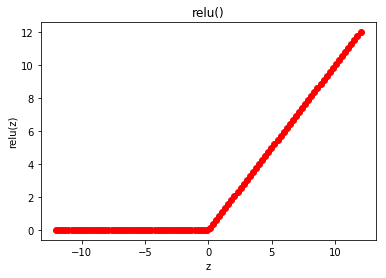
\includegraphics[scale=0.6]{figures/relu.png}
\end{block}
\end{frame}

\begin{frame}{The ReLU Transfer Function}
\begin{block}{Rectified Linear Unit (ReLU):}
\[ g(z) = \{ z \textrm{ if } z \geq 0 \textrm{ or } 0 \textrm{ if } z < 0 \} \]
or equivalently $g(z) = \textrm{max}\{0,z\}$
\end{block}

\pause
\begin{block}{Derivative of ReLU:}
\[ \frac{d g(z)}{dz} = \{ 1 \textrm{ if } z > 0 \textrm{ or } 0 \textrm{ if } z < 0 \} \]
non-differentiable or undefined if $z = 0$ \\
(in practice: choose a value for $z = 0$)
\end{block}
\end{frame}

\begin{frame}{The tanh Transfer Function $[-1,1]$}
\begin{block}{}
\centering
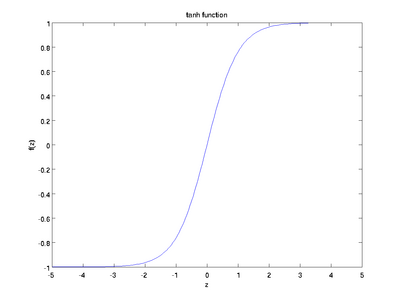
\includegraphics[scale=0.6]{figures/tanh.png}
\end{block}
\end{frame}

\begin{frame}{The tanh Transfer Function}
\begin{block}{tanh transfer function:}
\[ g(z) = \frac{e^{2z} - 1}{e^{2z} + 1} \]
\end{block}

\pause
\begin{block}{Derivative of tanh:}
\[ \frac{d g(z)}{dz} = 1 - g(z)^2 \]
\end{block}
\end{frame}

\begin{frame}{Derivatives w.r.t.\ parameters}
\begin{block}{Derivatives w.r.t.\ $w$:}
Given 
\[ h = g(w \cdot x + b) \]

derivatives w.r.t.\ $w_1, \ldots, w_j, \ldots w_d$:

\[ \frac{dh}{dw_j} \]
\end{block}

\pause
\begin{block}{Derivatives w.r.t.\ $b$:}
derivatives w.r.t.\ $b$:
\[ \frac{dh}{db} \]
\end{block}
\end{frame}

\begin{frame}{tanh Gradient}
\begin{block}{}
\centering
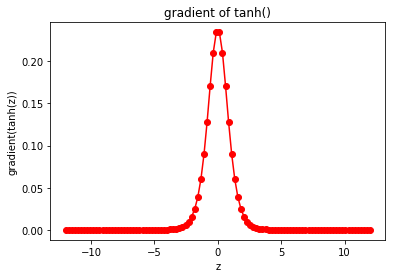
\includegraphics[scale=0.6]{figures/tanhgradient.png}
\end{block}
\end{frame}

\begin{frame}{Activation Functions and their Gradients}
\framesubtitle{from Goldberg 2017, Fig.\ 4.3}
\begin{block}{}
\centering
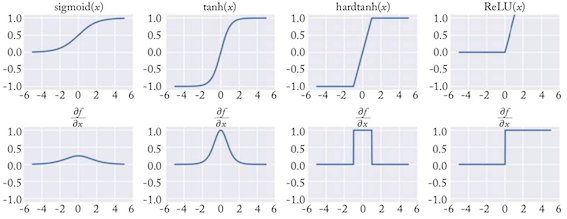
\includegraphics[scale=0.55]{figures/activationfns.png}
\end{block}
\end{frame}

\begin{frame}{Chain Rule of Differentiation}
\begin{block}{}
Introduce an intermediate variable $z \in \mathbb{R}$ 

\[ z = w \cdot x + b \]
\[ h = g(z) \]

Then by the chain rule to differentiate w.r.t.\ $w$:

\[ \frac{dh}{dw_j} = \textcolor{blue}{\frac{dh}{dz}} \textcolor{red}{\frac{dz}{dw_j}} = \textcolor{blue}{\frac{dg(z)}{dz}} \times \textcolor{red}{x_j}\]

\pause
And similarly for $b$:

\[ \frac{dh}{db} = \textcolor{blue}{\frac{dh}{dz}} \textcolor{red}{\frac{dz}{db}}= \textcolor{blue}{\frac{dg(z)}{dz}} \times \textcolor{red}{1}\]

\end{block}
\end{frame}

\begin{frame}{Single Layer Feedforward model}
\begin{block}{A single layer feedforward model consists of:}
\begin{itemize}[<+->]
\item An integer $d$ specifying the input dimension. Each input to the network is $x \in \mathbb{R}^d$
\item An integer $m$ specifying the number of hidden units
\item A parameter matrix $W \in \mathbb{R}^{m \times d}$. The vector $W_k \in \mathbb{R}^d$ for $1 \leq k \leq m$ is the $k$th row of $W$
\item A vector $b \in \mathbb{R}^d$ of bias parameters
\item A transfer function $g : \mathbb{R} \rightarrow \mathbb{R}$\\
$g(z) = \textrm{ReLU}(z)$ or $g(z) = \textrm{tanh}(z)$
\end{itemize}
\end{block}
\end{frame}

\begin{frame}{Single Layer Feedforward model (continued)}
\begin{block}{For $k = 1, \ldots, m$:}
\begin{itemize}[<+->]
\item The input to the $k$th neuron is: 
\( z_k = W_k \cdot x + b_k \)
\item The output from the $k$th neuron is: 
\( h_k = g(z_k) \)
\item Define vector $\phi(x; \theta) \in \mathbb{R}^m$ as:
\( \phi(x; \theta) = h_k \)
\item $\theta = (W, b)$ where $W \in \mathbb{R}^{m \times d}$ and $b \in \mathbb{R}^d$
\item Size of $\theta$ is $m \times (d+1)$ parameters 
\end{itemize}
\end{block}
\pause
\begin{block}{Some intuition}
The neural network employs $m$ hidden units, each with their own parameters $W_k$ and $b_k$, and these neurons are used to construct a \textit{hidden} representation $h \in \mathbb{R}^m$
\end{block}
\end{frame}

\begin{frame}{Matrix Form}
\begin{block}{}
We can replace the operation:

\[ z_k = W_k \cdot x + b \textrm{ for } k = 1, \ldots, m \]

with

\[ z = Wx + b \]

where the dimensions are as follows (vector of size $m$ equals a matrix of size $m \times 1$):

\[ \underbrace{z}_{m \times 1} = \underbrace{\underbrace{W}_{m \times d} \underbrace{x}_{d \times 1}}_{m \times 1} + \underbrace{b}_{m \times 1} \]

\end{block}
\end{frame}

\begin{frame}{Single Layer Feedforward model (matrix form)}
\begin{block}{A single layer feedforward model consists of:}
\begin{itemize}[<+->]
\item An integer $d$ specifying the input dimension. Each input to the network is $x \in \mathbb{R}^d$
\item An integer $m$ specifying the number of hidden units
\item A parameter matrix $W \in \mathbb{R}^{m \times d}$
\item A vector $b \in \mathbb{R}^d$ of bias parameters
\item A transfer function $g : \mathbb{R}^m \rightarrow \mathbb{R}^m$\\
$g(z) = [ \ldots, \textrm{ReLU}(z_i), \ldots ]$ or $g(z) = [ \ldots, \textrm{tanh}(z_i), \ldots ]$ for $i = 1, \ldots, m$
\end{itemize}
\end{block}
\end{frame}

\begin{frame}{Single Layer Feedforward model (matrix form, continued)}
\begin{block}{Define $\phi$ in matrix form:}
\begin{itemize}[<+->]
\item Vector of inputs to the hidden layer $z \in \mathbb{R}^m$: $z = Wx + b$
\item Vector of outputs from hidden layer $h \in \mathbb{R}^m$: $h = g(z)$
\item Define $\phi(x; \theta) = h$ where $\theta = (W, b)$
\[ \phi(x; \theta) = g(Wx + b) \]
\item Define $\textrm{softmax}_y(r) = \frac{exp(r_y)}{\sum_{y'} exp(r_{y'})}$ for $r \in \mathbb{R}^m$
\end{itemize}
\end{block}
\pause
\begin{block}{Putting it all together:}
\begin{eqnarray*}
\Pr(y \mid x; \theta, v) &=& \frac{exp\left(v(y) \cdot \phi(x;\theta) + \gamma_y \right)}{\sum_{y' \in {\cal Y}} exp\left(v(y') \cdot \phi(x;\theta) + \gamma_{y'})\right)} \\
 &=& \underbrace{\textrm{softmax}(\underbrace{v(y) \cdot \phi(x;\theta) + \gamma_y}_{\text{for each $y \in {\cal Y}$ an $\mathbb{R}$ value}})}_{\text{A vector of size $\mathbb{R}^{{\cal Y}}$ that sums to $1$}}
\end{eqnarray*}
\end{block}

\end{frame}

\begin{frame}{Feedforward neural network}
\begin{block}{}
\centering
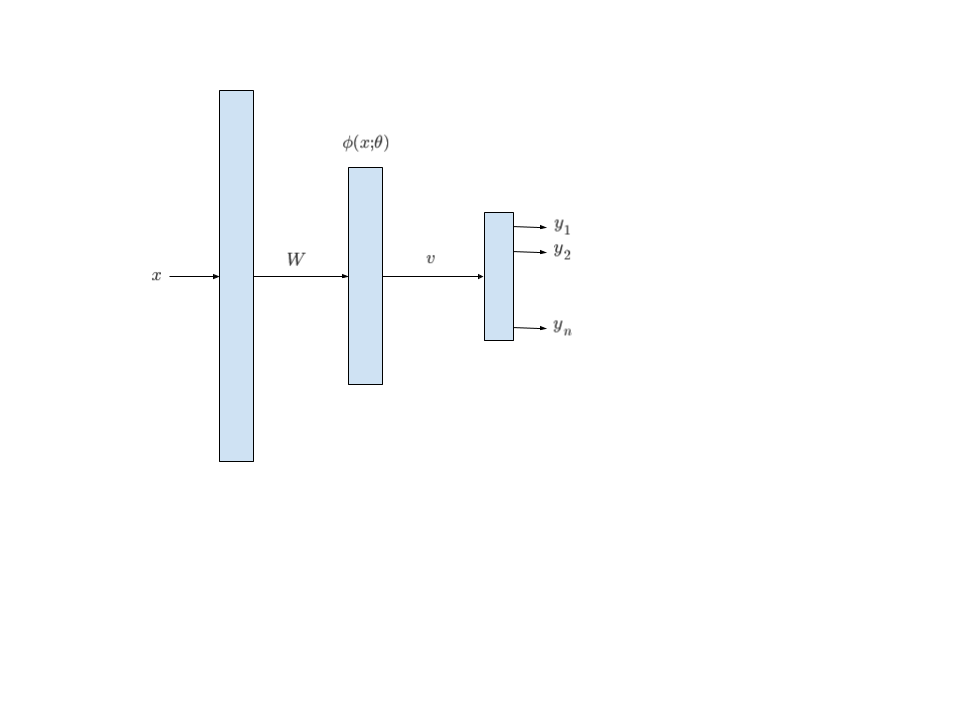
\includegraphics[scale=0.4]{figures/ffnet.png}
\end{block}
\end{frame}

\begin{frame}{n-gram Feedforward neural network}
\framesubtitle{(Bengio and Schwenk 2013)}
\begin{block}{}
\centering
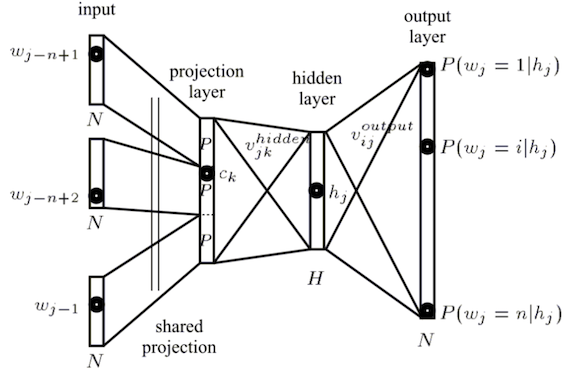
\includegraphics[scale=0.4]{figures/ngramfflm.png}
\end{block}
\end{frame}

\section{Stochastic Gradient Descent}
\frame{\tableofcontents[currentsection]}

\begin{frame}{Simple stochastic gradient descent}
\begin{block}{Inputs:}
\begin{itemize}[<+->]
\item Training examples $(x^i, y^i)$ for $i = 1, \ldots, n$
\item A feedforward representation $\phi(x; \theta)$
\item Integer $T$ specifying the number of updates
\item A sequence of learning rates: $\eta^1, \ldots, \eta^T$ where $\eta^t \in [0,1]$
\begin{itemize}[<+->]
\item One should experiment with learning rates: 0.001, 0.01, 0.1, 1
\item Bottou (2012) suggests a learning rate $\eta^t = \frac{\eta^1}{1 + \eta^1 \times \lambda \times t}$ where $\lambda$ is a hyperparameter that can be tuned experimentally
\end{itemize}
\end{itemize}
\end{block}
\pause
\begin{block}{Initialization:}
Set $v = (v(y), \gamma_y)$ for all $y$, and $\theta$ to random values
\end{block}
\end{frame}

\begin{frame}{Gradient descent}
\begin{block}{Algorithm:}
\begin{itemize}[<+->]
\item For $t = 1, \ldots, T$
\begin{itemize}[<+->]
\item Select an integer $i$ uniformly at random from $\{ 1, \ldots, n \}$
\item Define $L(\theta, v) = - \log P(y_i \mid x_i; \theta, v)$
\item For each parameter $\theta_j$ and $v_k(y)$ and $\gamma_y$ (for each label $y$):
\begin{eqnarray*}
\theta_j &=& \theta_j - \eta^t \times \frac{dL(\theta,v)}{d\theta_j} \\
v_k(y) &=& v_k(y) - \eta^t \times \frac{dL(\theta,v)}{d v_k(y)} \\
\gamma(y) &=& \gamma(y) - \eta^t \times \frac{dL(\theta,v)}{d \gamma(y)}
\end{eqnarray*}
\end{itemize}
\item \textbf{Output}: parameters $\theta$, $v = (v(y), \gamma_y)$ for all $y$
\end{itemize}
\end{block}
\end{frame}

\section{Motivating example: XOR}
\frame{\tableofcontents[currentsection]}

\begin{frame}{Motivating example: the XOR problem}
\begin{block}{From \textit{Deep Learning} by Goodfellow, Bengio, Courville}
We will assume a training set where each label is in the set ${\cal Y} = \{ -1, +1 \}$

There are four training examples:
\begin{eqnarray*}
x^1 &=& [0,0], y^1 = -1\\
x^2 &=& [0,1], y^2 = +1 \\
x^3 &=& [1,0], y^3 = +1\\
x^4 &=& [1,1], y^4 = -1
\end{eqnarray*}
\end{block}
\end{frame}

\begin{frame}{Motivating example: the XOR problem}
\begin{block}{}
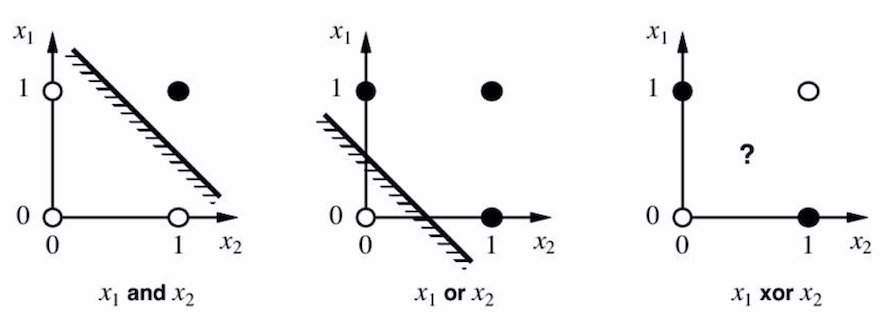
\includegraphics[scale=0.7]{figures/xorfig.png}
\end{block}
\end{frame}

\begin{frame}{Motivating example: the XOR problem}
\begin{block}{Theorem}
For examples $(x^i, y^i)$ for $i = 1,\ldots,4$ as defined previously for the feedforward neural network:
\[ \Pr(y \mid x; W, b, v) = \frac{exp\left(v(y) \cdot g(Wx + b) + \gamma_y \right)}{\sum_{y' \in {\cal Y}} exp\left(v(y') \cdot g(Wx + b) + \gamma_{y'})\right)} \]
where $x \in \mathbb{R}^2$ ($d=2$) and let $m=2$ so $W \in \mathbb{R}^{2\times2}$ and $b \in \mathbb{R}^2$ and $g$ is a ReLU transfer function.

\pause
Then there are parameter settings $v(-1)$, $v(+1)$, $\gamma_{-1}$, $\gamma_{+1}$, $W, b$ such that 

\[ p(y^i \mid x^i; v) > 0.5 \textrm{   for } i = 1, \ldots, 4 \]
\end{block}
\end{frame}

\begin{frame}{Motivating example: the XOR problem}
\begin{block}{Proof Sketch}
Define $W = \begin{bmatrix}
 1 & 1 \\
 1 & 1 
 \end{bmatrix}$ 
and $b = \begin{bmatrix} 0 \\ -1 \end{bmatrix}$
\pause
Then for each input $x$ calculate values of $z = Wx+b$ and $h=g(z)$:

\begin{eqnarray*}
x = [0,0] &\Rightarrow& z = [0,-1] \Rightarrow h = [0,0] \\
x = [1,0] &\Rightarrow& z = [1,0] \Rightarrow h = [1,0] \\
x = [0,1] &\Rightarrow& z = [1,0] \Rightarrow h = [1,0] \\
x = [1,1] &\Rightarrow& z = [2,1] \Rightarrow h = [2,1] 
\end{eqnarray*}
\end{block}
\end{frame}

\begin{frame}{Motivating example: the XOR problem}
\begin{block}{Proof Sketch (continued)}
\begin{eqnarray*}
p(+1 \mid x; v) &=& \frac{exp(v(+1) \cdot h  + \gamma_{+1})}{exp(v(+1) \cdot h  + \gamma_{+1}) + exp(v(-1) \cdot h + \gamma_{-1})} \\
&=& \frac{1}{1 + exp(-(u \cdot h + \gamma))}
\end{eqnarray*}

\pause
To satisfy $P(y^i \mid x^i; v) > 0.5$ for $i = 1,\ldots,4$
we have to find parameters $u = v(+1) - v(-1)$ and $\gamma = \gamma_{+1} - \gamma_{-1}$
such that:

\begin{eqnarray*}
u \cdot [0,0] + \gamma &<& 0 \\
u \cdot [1,0] + \gamma &>& 0 \\
u \cdot [1,0] + \gamma &>& 0 \\
u \cdot [2,1] + \gamma &<& 0
\end{eqnarray*}

$u = [1, -2]$ and $\gamma = -0.5$ satisfies these constraints.
\end{block}
\end{frame}

\begin{frame}{Solving the XOR problem}
\begin{figure}
   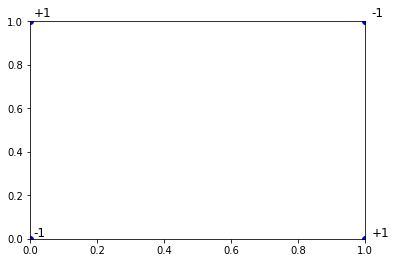
\includegraphics[width=0.475\textwidth]{figures/xorbefore.png}
   \hfill
   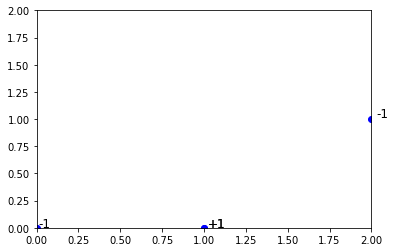
\includegraphics[width=0.475\textwidth]{figures/xorafter.png}
\end{figure}
\end{frame}


\section*{Acknowledgements}

\begin{frame}
\centering
\begin{alertblock}{Acknowledgements}
Many slides borrowed or inspired from lecture notes by Michael Collins, Chris Dyer, Kevin Knight, Philipp Koehn, Adam Lopez, Graham Neubig and Luke Zettlemoyer from their NLP course materials. 

\bigskip

All mistakes are my own.

\bigskip

A big thank you to all the students who read through these notes and helped me improve them.

\end{alertblock}
\end{frame}



\end{document}
 
 
